\documentclass[11pt,a4paper]{article}

\usepackage[T1]{fontenc}
\usepackage[utf8]{inputenc}
\usepackage[italian]{babel}
\usepackage{amsmath,amssymb}
\usepackage[a4paper,margin=2.5cm]{geometry}
\usepackage{array}
\usepackage{siunitx}
\usepackage{booktabs}
\usepackage{graphicx}
\usepackage{float}
\usepackage{hyperref}

\hypersetup{hidelinks}
\setlength{\parindent}{0pt}
\setlength{\parskip}{4pt}
\allowdisplaybreaks
\graphicspath{{figure/}}
\sisetup{output-decimal-marker={,}, group-separator={\,}, per-mode=symbol,
         exponent-product=\cdot, range-phrase={\text{--}}}

\newcommand{\uma}{u-a}
\newcommand{\upa}{u+a}
\newcommand{\Ru}{R_1}
\newcommand{\Rd}{R_2}
\newcommand{\Me}{M_e}
\newcommand{\Mst}{M^{*}}

\title{Gasdinamica -- Svolgimento esercizio 2 (B70-E02)\\[2pt]
\large Condizione al contorno per lo scarico di un tubo}
\author{}
\date{Prova del 13/02/2023}

\begin{document}
\maketitle

\section*{Traccia}
\emph{Boundary condition for pipe discharge (score 8/30).} The exit section boundary condition for an unsteady
omentropic subsonic airflow along a pipe is
\[
  \frac{\gamma+1}{2}\left(\frac ua\right)^{\frac{4}{\gamma+1}}+\left(\frac au\right)^{\frac{2(\gamma-1)}{\gamma+1}}=K,
\]
with $K=\text{const.}>1$, $u$ and $a$ the velocity and the speed of sound, respectively, at the exit section.
Evaluate its effect on an acoustic simple wave propagating toward the exit section from inside the pipe.

%==============================================================================
\section{Lettura del testo e dati}
Il tubo scarica: la corrente va verso la sezione d'uscita, che pongo all'estremo destro $x=L$, quindi
$0<u<a$ in uscita. La condizione lega $u$ e $a$ solo attraverso il loro rapporto $M=u/a$:
\[
  f(M)\equiv\frac{\gamma+1}{2}\,M^{\frac{4}{\gamma+1}}+M^{-\frac{2(\gamma-1)}{\gamma+1}}=K .
\]
Dall'interno arriva un'onda semplice \emph{acustica}, cioè di piccola ampiezza: va determinato che cosa
riflette il contorno, cioè natura e intensità dell'onda riflessa rispetto all'incidente. La traccia non dà
valori numerici: il risultato si ottiene in forma generale. Per i valori numerici di confronto uso l'aria
($\gamma=\num{1.4}$, $\delta=(\gamma-1)/2=\num{0.2}$).

%==============================================================================
\section{Modello e ipotesi}
\begin{itemize}
  \item \textbf{Eulero 1D instazionario omoentropico}, come dice la traccia: il tubo ha sezione costante e le onde
    sono piane. L'omoentropia rende validi ovunque gli invarianti di Riemann
    $\Ru=a-\delta u$, costante lungo le caratteristiche $\uma$, e $\Rd=a+\delta u$, costante lungo le $\upa$.
  \item \textbf{Onda incidente semplice della famiglia $\upa$}: è l'unica famiglia che dall'interno raggiunge il
    contorno destro. In essa $\Ru$ è uniforme ($da=\delta\,du$).
  \item \textbf{Stato 0 uniforme} davanti all'onda incidente, che soddisfa già la condizione d'uscita (flusso di
    scarico precedente all'arrivo dell'onda).
  \item \textbf{Piccola ampiezza}: le onde restano continue e non si formano urti nel tratto considerato, quindi
    l'omoentropia si conserva anche dopo la riflessione.
\end{itemize}

%==============================================================================
\section{Analisi qualitativa}
L'onda incidente $\upa$, arrivando all'uscita, varia lo stato nella sezione. Il contorno non può assorbirla
liberamente: poiché fissa il rapporto $u/a$, la velocità di uscita può crescere solo in proporzione alla velocità
del suono. Nasce quindi un'onda riflessa della famiglia $\uma$, che risale il tubo verso l'interno.

Il contorno ha un comportamento intermedio tra quelli noti. Per una compressione incidente:
\begin{itemize}
  \item su una \emph{parete} ($u=0$) il gas non può accelerare e la compressione si riflette come compressione di
    pari intensità;
  \item su un \emph{estremo aperto} ($p$ imposta) la pressione non può crescere e si riflette un'espansione;
  \item qui il gas accelera, ma meno di quanto chiederebbe l'estremo aperto, perché $u$ deve restare $\Me a$.
    L'eccesso di pressione non scaricato torna indietro: mi aspetto una riflessa \textbf{della stessa natura}
    dell'incidente e \textbf{più debole}, come per un estremo ``parzialmente chiuso''.
\end{itemize}
Per un'espansione incidente il ragionamento è speculare: si riflette un'espansione.

%==============================================================================
\section{Topologia del campo}
Nel piano $x$--$t$ (figura~\ref{fig:xt}) si distinguono:
\begin{itemize}
  \item \textbf{stato 0}, uniforme, davanti all'onda incidente;
  \item \textbf{onda incidente} $\upa$, semplice ($\Ru=\Ru_{,0}$ uniforme), e dietro di essa lo \textbf{stato 1};
  \item una \textbf{zona d'interazione a due famiglie} a ridosso dell'uscita, di durata pari al tempo di
    passaggio dell'onda incidente;
  \item \textbf{onda riflessa} $\uma$, semplice ($\Rd=\Rd_{,1}$ uniforme), che risale il tubo nello stato 1;
  \item \textbf{stato 2}, uniforme, tra l'onda riflessa e la sezione d'uscita.
\end{itemize}

%==============================================================================
\section{Bilancio equazioni/incognite}
Nella sezione d'uscita subsonica ($0<u<a$) le caratteristiche $\upa$ e $u$ escono dal dominio, la $\uma$ vi
entra: serve \textbf{una} condizione al contorno, e la relazione $f(M)=K$ è proprio una relazione scalare.
Le incognite al contorno sono $a$ e $u$. Le equazioni sono due: la compatibilità lungo la $\upa$ che arriva
dall'interno (che porta $\Rd$) e la condizione $f(M)=K$. Il problema è ben posto.

%==============================================================================
\section{Scorciatoie fisiche}
La condizione contiene solo $M$ e $K$ è costante, quindi nella sezione d'uscita
\[
  M=\frac ua=\Me=\text{cost.},
\]
con $\Me$ radice di $f(M)=K$: la condizione equivale a imporre il numero di Mach d'uscita, come avviene per
uno scarico attraverso un restringimento strozzato. Lo stesso risultato si ottiene derivando nel tempo. Gli esponenti soddisfano $\frac{4}{\gamma+1}+\frac{2(\gamma-1)}{\gamma+1}=2$,
quindi
\[
  \frac{d f}{dt}=f'(M)\,M_t=0,\qquad
  f'(M)=2M^{-\frac{3\gamma-1}{\gamma+1}}\left(M^2-\frac{\gamma-1}{\gamma+1}\right),\qquad
  M_t=\frac{u_t-M a_t}{a},
\]
cioè
\[
  \left(M^2-\frac{\gamma-1}{\gamma+1}\right)\left(u_t-M a_t\right)=0
  \quad\Rightarrow\quad u_t-M a_t=0 .
\]
Restano esclusi $M=0$ (dove $f\to\infty$), $M=1$ (dove la $\uma$ non entra più) e
$M=\Mst=\sqrt{(\gamma-1)/(\gamma+1)}$, discusso nel \S\,\ref{sec:fM}.

%==============================================================================
\section{Calcolo}

\subsection{Stati d'uscita ammessi}\label{sec:fM}
$f(M)\to\infty$ per $M\to0$ e $f'$ si annulla solo in $\Mst$, dove $f$ ha il minimo:
\[
  \Mst=\sqrt{\frac{\gamma-1}{\gamma+1}}=\num{0.408},\qquad
  f(\Mst)=\frac{\gamma+1}{2}\left(\frac{\gamma+1}{\gamma-1}\right)^{\frac{\gamma-1}{\gamma+1}}
  =\num{1.2}\cdot 6^{1/6}=\num{1.62},
\]
\[
  f(1)=\frac{\gamma+3}{2}=\num{2.2}.
\]
Quindi $K>1$ è necessario ma non basta. Per l'aria:
\begin{itemize}
  \item $1<K<\num{1.62}$: nessuno stato d'uscita soddisfa la condizione;
  \item $\num{1.62}<K<\num{2.2}$: due radici subsoniche, $M_a<\Mst<M_b<1$;
  \item $K>\num{2.2}$: una sola radice subsonica $M_a<\Mst$, perché l'altra è supersonica ed è esclusa
    dall'ipotesi di uscita subsonica.
\end{itemize}
Vale la radice del flusso di scarico iniziale. Poiché $M$ al contorno varia con continuità, non può saltare
all'altra radice. Per $K=f(\Mst)$ la radice è doppia e la forma differenziale degenera, ma $f>K$ per ogni
$M\neq\Mst$, quindi anche lì $M=\Mst$ resta fisso. Per esempio, con $K=\num{1.8}$ le radici, trovate per
tentativi, sono $M_a\approx\num{0.196}$ e $M_b\approx\num{0.711}$.

\subsection{Condizione in termini di invarianti}
Con $u=\Me a$ nella sezione d'uscita:
\[
  \Ru=a(1-\delta\Me),\qquad \Rd=a(1+\delta\Me)
  \quad\Rightarrow\quad
  \Ru\big|_{e}=\frac{1-\delta\Me}{1+\delta\Me}\,\Rd\big|_{e}.
\]
La relazione è esatta e lineare: l'invariante che entra nel tubo è proporzionale a quello che arriva
dall'interno.

\subsection{Stati 0, 1, 2}
\textbf{Stato 0.} Soddisfa il contorno: $u_0=\Me a_0$ e $\Ru_{,0}=\frac{1-\delta\Me}{1+\delta\Me}\Rd_{,0}$.

\textbf{Stato 1} (dietro l'onda incidente $\upa$). $\Ru_{,1}=\Ru_{,0}$, mentre $\Rd$ varia di $\Delta\Rd$, che
misura l'intensità dell'incidente:
\[
  \Delta a_i=a_1-a_0=\tfrac12\Delta\Rd,\qquad \Delta u_i=u_1-u_0=\frac{\Delta a_i}{\delta}.
\]

\textbf{Stato 2} (dietro la riflessa $\uma$, sulla sezione d'uscita). Attraverso la riflessa
$\Rd_{,2}=\Rd_{,1}$; il contorno dà $\Ru_{,2}=\frac{1-\delta\Me}{1+\delta\Me}\Rd_{,1}$. Sottraendo la
relazione dello stato 0:
\[
  \Delta\Ru=\Ru_{,2}-\Ru_{,1}=\frac{1-\delta\Me}{1+\delta\Me}\,\Delta\Rd .
\]
Attraverso la riflessa $\Delta a_r=a_2-a_1=\tfrac12\Delta\Ru$ e $\Delta u_r=-\Delta a_r/\delta$, quindi
\[
  \boxed{\;\frac{\Delta a_r}{\Delta a_i}=\frac{\Delta\Ru}{\Delta\Rd}=\frac{1-\delta\Me}{1+\delta\Me}\;}
  \qquad 0<\frac{1-\delta\Me}{1+\delta\Me}<1 \ \text{per}\ 0<\Me<1 .
\]
Per un'onda acustica $\Delta p/p=\frac{2\gamma}{\gamma-1}\,\Delta a/a$, quindi lo stesso rapporto vale per le
perturbazioni di pressione: $\Delta p_r/\Delta p_i=(1-\delta\Me)/(1+\delta\Me)$.
Nella sezione d'uscita le variazioni complessive sono
\[
  a_2-a_0=\frac{2\,\Delta a_i}{1+\delta\Me},\qquad
  u_2-u_0=\frac{2\delta\Me}{1+\delta\Me}\,\Delta u_i ,
\]
cioè $a$ cresce quasi quanto su una parete ($2\Delta a_i$) e $u$ molto meno che su un estremo aperto
($2\Delta u_i$).

\subsection{Forma differenziale: gradienti delle onde}\label{sec:diff}
Le relazioni caratteristiche danno al contorno
\[
  a_t=-\frac{u+a}{2}\,(a+\delta u)_x-\frac{u-a}{2}\,(a-\delta u)_x,\qquad
  u_t=-\frac{u+a}{2\delta}\,(a+\delta u)_x+\frac{u-a}{2\delta}\,(a-\delta u)_x .
\]
Sostituendo in $u_t-Ma_t=0$, con $u=Ma$:
\[
  (a-\delta u)_x=-\frac{(1+M)(1-\delta M)}{(1-M)(1+\delta M)}\,(a+\delta u)_x .
\]
Nell'onda incidente $\upa$ si ha $(a+\delta u)_x=2a_{x,i}$, nella riflessa $\uma$ $(a-\delta u)_x=2a_{x,r}$, quindi
\[
  a_{x,r}=-\frac{(1+\Me)(1-\delta\Me)}{(1-\Me)(1+\delta\Me)}\;a_{x,i}.
\]
Una compressione incidente $\upa$ ha $a_{x,i}<0$ (il gas più ``caldo'' sta dietro, a sinistra), quindi
$a_{x,r}>0$: la riflessa $\uma$ ha il gas compresso dietro di sé, a destra, ed è una \textbf{compressione}.
Viceversa, un'espansione incidente si riflette come espansione. Il fattore $(1+\Me)/(1-\Me)$ rispetto al rapporto
delle ampiezze è il rapporto delle velocità di propagazione $(a+u)/(a-u)$. La riflessa ha la stessa durata
dell'incidente ma risale la corrente più lentamente, quindi è più corta nello spazio e più ripida. Per
$\Me\to0$ si ritrova $a_{x,r}=-a_{x,i}$, cioè la parete.

\subsection{Esempio numerico}
Aria, $K=\num{1.8}$ con la radice $\Me=M_b\approx\num{0.711}$, stato 0 di riferimento $p_0=1$, $a_0=1$, e
compressione incidente con $p_1/p_0=\num{1.10}$:
\begin{itemize}
  \item stato 1: $\Ru=a_0-\delta u_0=\num{0.858}$ uniforme,
    $a_1=a_0(p_1/p_0)^{(\gamma-1)/(2\gamma)}=\num{1.10}^{1/7}=\num{1.0137}$,
    $u_1=(a_1-\Ru)/\delta=\num{0.780}$;
  \item stato 2: $\Rd=a_1+\delta u_1=\num{1.170}$ uniforme, $a_2=\Rd/(1+\delta\Me)=\num{1.170}/\num{1.142}=\num{1.024}$,
    $u_2=\Me a_2=\num{0.728}$, $p_2=a_2^{7}=\num{1.181}$.
\end{itemize}
\begin{table}[H]
  \centering
  \begin{tabular}{cccccccc}
    \toprule
    Stato & $a/a_0$ & $u/a_0$ & $p/p_0$ & $M$ & $\Ru$ & $\Rd$ & $u-a$ \\
    \midrule
    0 & \num{1} & \num{0.711} & \num{1} & \num{0.711} & \num{0.858} & \num{1.142} & \num{-0.289} \\
    1 & \num{1.014} & \num{0.780} & \num{1.100} & \num{0.769} & \num{0.858} & \num{1.170} & \num{-0.234} \\
    2 & \num{1.024} & \num{0.728} & \num{1.181} & \num{0.711} & \num{0.878} & \num{1.170} & \num{-0.296} \\
    \bottomrule
  \end{tabular}
  \caption{Stati dell'esempio (aria, $\Me\approx\num{0.711}$, $p_1/p_0=\num{1.10}$).}
\end{table}
$\Delta a_r/\Delta a_i=\num{0.0103}/\num{0.0137}=\num{0.751}=(1-\num{0.142})/(1+\num{0.142})$, come previsto.
In pressione $\Delta p_r/\Delta p_i=\num{0.081}/\num{0.100}=\num{0.81}$, poco diverso perché un aumento del
\SI{10}{\percent} non è più strettamente acustico. Con la radice $M_a\approx\num{0.196}$ il rapporto sarebbe
$\num{0.924}$: a basso Mach il contorno è quasi una parete.

%==============================================================================
\section{Verifiche a posteriori}
\begin{itemize}
  \item Numero di condizioni: uscita subsonica, una caratteristica entrante, una condizione. \emph{Verificata.}
  \item Nessuna variabile d'onda uscente prescritta: la condizione fissa $\Ru$ (entrante) in funzione di $\Rd$
    (uscente) e non vincola $\Rd$. \emph{Verificata.}
  \item La riflessa entra nel tubo: $u-a=a(\Me-1)<0$; nell'esempio $u_2-a_2=\num{-0.296}$. \emph{Verificata.}
  \item Stato 2 sul contorno: $u_2/a_2=\num{0.728}/\num{1.024}=\num{0.711}=\Me$. \emph{Verificata.}
  \item Natura: compressione incidente, $\Delta a_r>0$, riflessa di compressione, come previsto nell'analisi
    qualitativa. \emph{Verificata.}
  \item Casi limite: per $\Me\to0$ il rapporto vale 1 (parete, $u=0$). Non vale mai $-1$ (estremo aperto) e si
    annullerebbe solo per $\Me=1/\delta=5$, quindi in subsonico il contorno non è mai non riflettente.
    \emph{Coerente.}
  \item Omoentropia: nessun urto per onde acustiche. La riflessa è più ripida dell'incidente, quindi per ampiezze
    finite raggiungerebbe prima la formazione dell'urto. \emph{Verificata nel limite acustico.}
\end{itemize}

%==============================================================================
\section{Risultati}
\begin{table}[H]
  \centering
  \renewcommand{\arraystretch}{1.7}
  \begin{tabular}{p{0.37\textwidth}p{0.38\textwidth}l}
    \toprule
    Grandezza & Valore & Natura \\
    \midrule
    Condizione equivalente & $u/a=\Me=\text{cost.}$, radice subsonica di $f(M)=K$ & esatto \\
    Esistenza dello stato d'uscita & $K\ge f(\Mst)$; aria $K\ge\num{1.62}$; due radici per $K<\num{2.2}$ & esatto \\
    Natura della riflessa ($\uma$) & stessa dell'incidente & esatto \\
    Intensità & $\Delta\Ru/\Delta\Rd=\Delta a_r/\Delta a_i=\dfrac{1-\delta\Me}{1+\delta\Me}$ & esatto \\
    Perturbazione di pressione & $\Delta p_r/\Delta p_i=\dfrac{1-\delta\Me}{1+\delta\Me}$ & limite acustico \\
    Gradienti & $a_{x,r}/a_{x,i}=-\dfrac{(1+\Me)(1-\delta\Me)}{(1-\Me)(1+\delta\Me)}$ & limite acustico \\
    Variazione in uscita & $\Delta a_e=\dfrac{2\Delta a_i}{1+\delta\Me}$,\ $\Delta u_e=\dfrac{2\delta\Me\,\Delta u_i}{1+\delta\Me}$ & esatto \\
    Esempio (aria, $K=\num{1.8}$) & $\Me\approx\num{0.711}$: \num{0.751};\ $\Me\approx\num{0.196}$: \num{0.924} & \\
    \bottomrule
  \end{tabular}
  \caption{Risultati.}
\end{table}

%==============================================================================
\section{Rappresentazioni}
\begin{figure}[H]
  \centering
  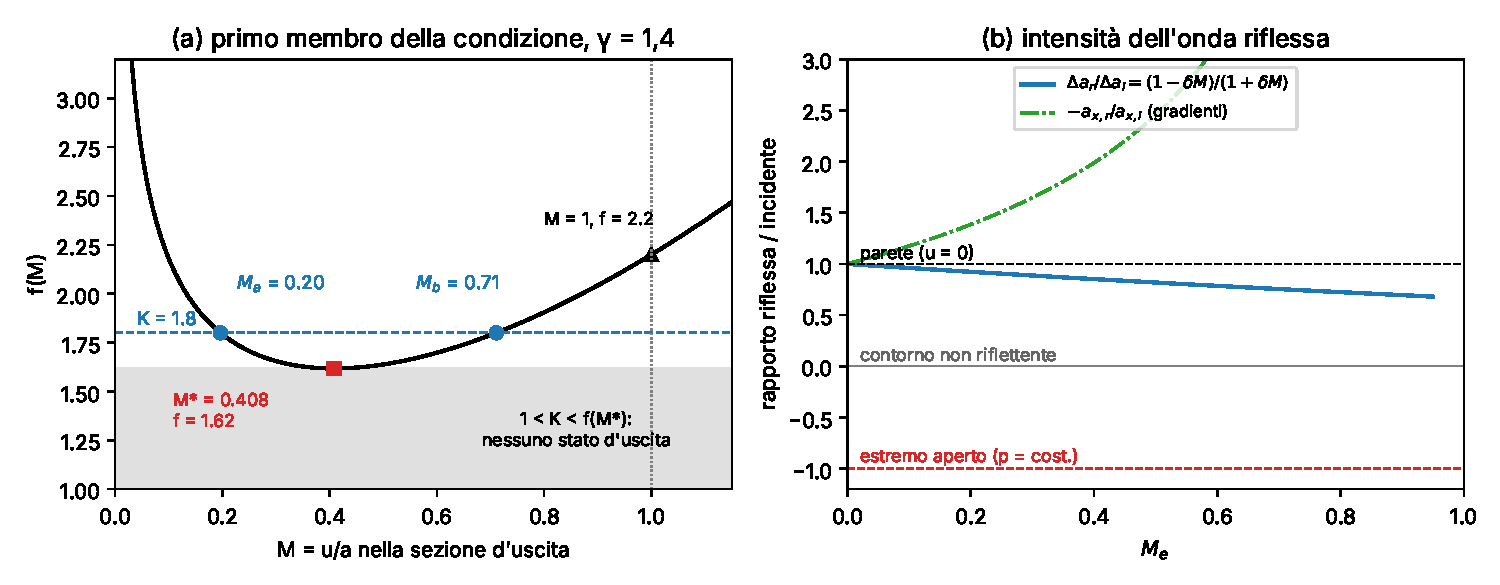
\includegraphics[width=\textwidth]{fM_rapporto.pdf}
  \caption{(a) Primo membro $f(M)$ della condizione per $\gamma=\num{1.4}$, con il minimo in $\Mst$ e le due radici
  per $K=\num{1.8}$. (b) Rapporto tra onda riflessa e incidente in funzione di $\Me$, confrontato con parete ed
  estremo aperto.}
  \label{fig:fM}
\end{figure}
La figura~\ref{fig:fM}(a) mostra perché $K>1$ non basta: la curva non scende sotto $f(\Mst)\approx\num{1.62}$,
e tra questo valore e $f(1)=\num{2.2}$ ogni livello $K$ taglia due rami subsonici. Nella (b) il rapporto delle
ampiezze resta tra $\num{0.67}$ e 1, sempre dalla parte della parete e mai dell'estremo aperto. Il rapporto dei
gradienti cresce invece rapidamente con $\Me$: la riflessa è molto più ripida dell'incidente quando la corrente
d'uscita è vicina al sonico.

\begin{figure}[H]
  \centering
  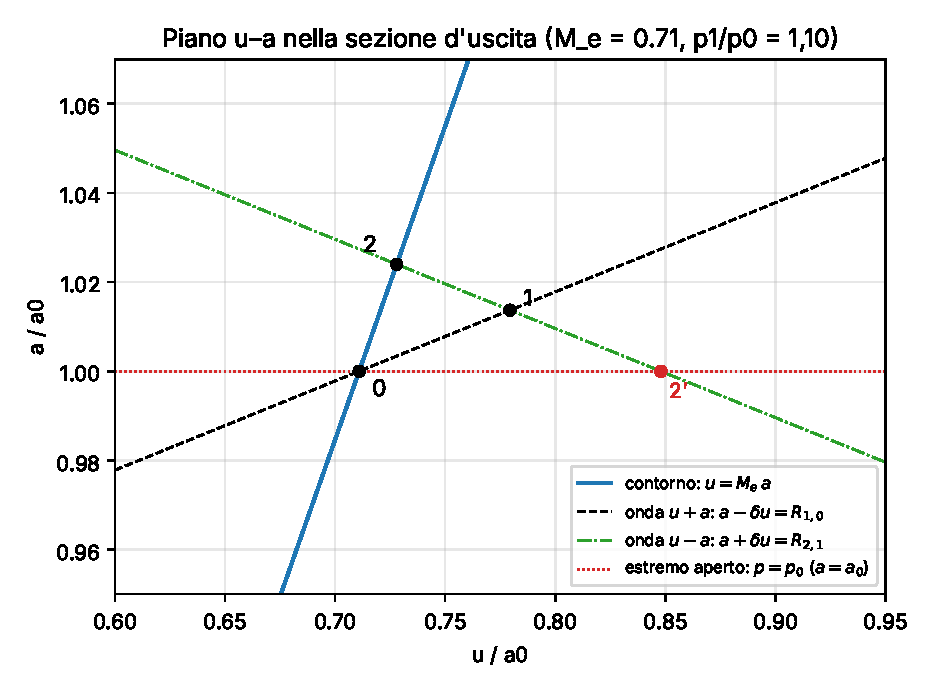
\includegraphics[width=0.66\textwidth]{piano_ua.pdf}
  \caption{Piano $u$--$a$ dell'esempio ($\Me\approx\num{0.711}$, $p_1/p_0=\num{1.10}$). Lo stato 2' è quello che
  si avrebbe con un estremo aperto ($p=p_0$).}
  \label{fig:ua}
\end{figure}
Nel piano $u$--$a$ (figura~\ref{fig:ua}) le onde semplici sono rette ($a\mp\delta u=\text{cost.}$) e il contorno è
la retta per l'origine $a=u/\Me$. Lo stato 1 sta sulla retta $\Ru=\Ru_{,0}$, lo stato 2 all'intersezione della
$\Rd=\Rd_{,1}$ con la retta del contorno. Poiché quest'ultima è ripida, lo stato 2 si trova sopra lo stato 1: la
riflessa è una compressione. Con l'estremo aperto (stato 2' su $a=a_0$) si scenderebbe invece sotto lo stato 1
e la riflessa sarebbe un'espansione. Il piano $u$--$a$ equivale al $p$--$u$ per un campo omoentropico, ma ha il
vantaggio di avere rette.

\begin{figure}[H]
  \centering
  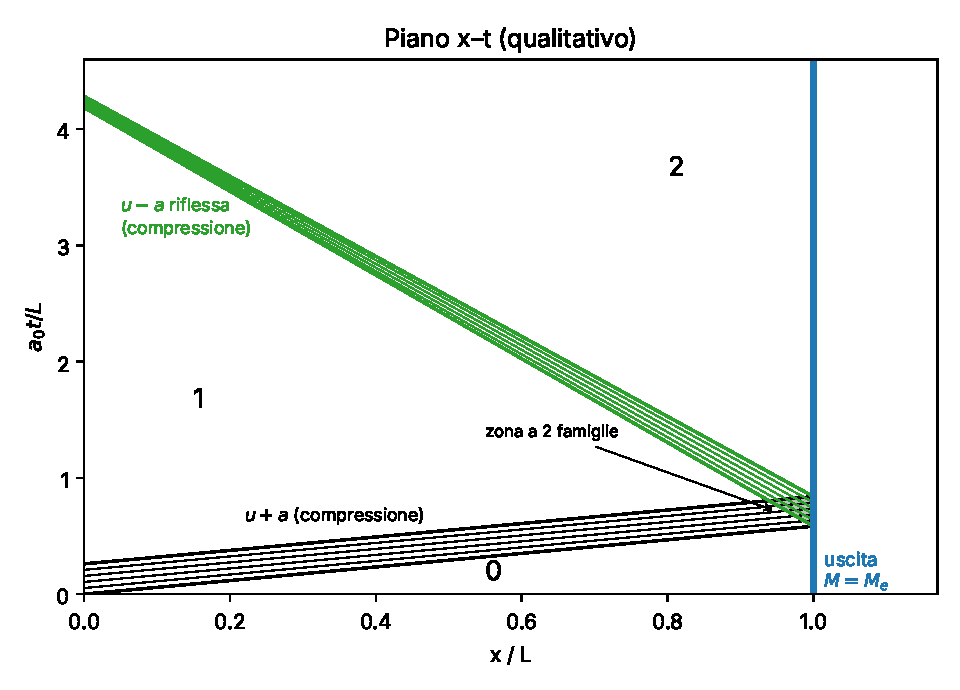
\includegraphics[width=0.7\textwidth]{xt.pdf}
  \caption{Piano $x$--$t$ qualitativo di un'onda acustica di compressione che si riflette all'uscita
  ($\Me\approx\num{0.711}$). Le caratteristiche sono tracciate come semirette con le pendenze degli stati uniformi.}
  \label{fig:xt}
\end{figure}
Nel piano $x$--$t$ (figura~\ref{fig:xt}) l'onda incidente $\upa$ arriva all'uscita in un intervallo di tempo
finito. La riflessa $\uma$ parte dall'uscita nello stesso intervallo, ma risale la corrente con velocità
$|u-a|\approx\num{0.29}\,a_0$ contro $u+a\approx\num{1.7}\,a_0$ dell'incidente, quindi occupa un tratto di tubo
molto più corto. La zona a due famiglie a ridosso dell'uscita non va risolta. Si potrebbe risolvere con le
relazioni di compatibilità e la condizione $u=\Me a$; sulla sezione d'uscita $a$ e $p$ vi crescono con continuità
dal valore dello stato 0 a quello dello stato 2.

%==============================================================================
\section{Discussione fisica}
La condizione assegnata equivale a imporre il numero di Mach in uscita. Il caso fisico tipico è lo scarico
attraverso un restringimento strozzato, dove il rapporto tra la sezione del tubo e quella critica fissa $\Me$.
Questo contorno riflette le onde \textbf{senza cambiarne la natura} e le attenua solo del fattore
$(1-\delta\Me)/(1+\delta\Me)$: è un'estremità ``quasi chiusa''. Il comportamento coincide con quello dell'uscita
strozzata nello svuotamento di un tubo, dove l'espansione proveniente dalla parete torna indietro ancora come
espansione. La parte non riflessa dell'onda esce dal tubo come variazione della portata, che cresce con $a$
($\dot m\propto\rho a\Me\propto a^{(\gamma+1)/(\gamma-1)}$).

In un tubo chiuso all'altro estremo, un disturbo rimbalzerebbe quindi tra parete e uscita perdendo a ogni
riflessione all'uscita solo una frazione $2\delta\Me/(1+\delta\Me)$ della sua ampiezza: lo smorzamento è lento,
soprattutto a basso $\Me$, e il tubo può risuonare. All'opposto, l'estremo aperto inverte la natura delle onde.
Infine, la riflessa è più ripida dell'incidente del fattore $(1+\Me)/(1-\Me)$. Per ampiezze non piccole, le
compressioni riflesse tendono a degenerare in urto prima dell'incidente, e lì il modello omoentropico smette di
valere.

\end{document}
